\begin{figure}
  \begin{subfigure}[b]{\textwidth}
    \centering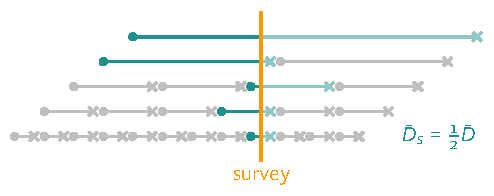
\includegraphics[scale=1]{diag.yss.censor}
    \caption{Right censoring of reported durations selling sex in a steady state population}
    \label{fig:diag.yss.censor}
  \end{subfigure}
  \begin{subfigure}[b]{\textwidth}
    \centering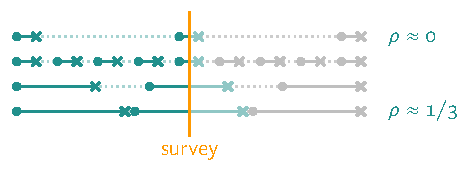
\includegraphics[scale=1]{diag.yss.gaps}
    \caption{Possible periods of selling sex for one respondent who stopped 0, 1, or 2 times}
    \label{fig:diag.yss.gaps}
  \end{subfigure}
  \begin{subfigure}[b]{\textwidth}
    \centering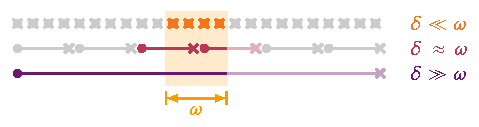
\includegraphics[scale=1]{diag.partner.cases}
    \caption{Differences in partnership duration \vs recall period}
    \label{fig:diag.partner.cases}
  \end{subfigure}
  \begin{subfigure}[b]{\textwidth}
    \centering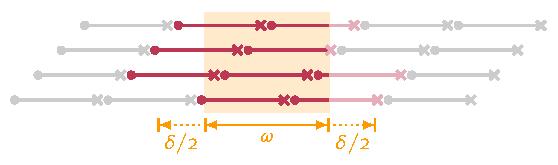
\includegraphics[scale=1]{diag.partner.recall}
    \caption{Fully and partially observed partnerships during a given recall period}
    \label{fig:diag.partner.recall}
  \end{subfigure}
  \caption{Diagrams of fully observed, censored, and unobserved periods
    selling sex or within ongoing sexual partnerships}
  \label{fig:diag}
  \floatfoot{Guide:
    \g{$\bullet$\,}{start}, \g{$\bm{\times}$\,}{end},
    \g{yellow}{survey/recall period},
    \g{full colour}{fully observed}, \g{faded colour}{right censored}, \g{grey}{unobserved},
    \g{$\bar{d}$}{mean duration at survey} and \g{$\bar{D}$}{overall},
    \g{$s$}{number of times stopped selling sex}, \g{$g$}{relative gap length \vs $D$},
    \g{$\omega$}{recall period}, \g{$\delta$}{partnership duration},
    \g{$x$}{number of reported partnerships}.}
\end{figure}